% Document
\documentclass{article}

% Packages
\usepackage[utf8]{inputenc}                                                             % input encoding
\usepackage[T1]{fontenc}                                                                % font encoding
\usepackage[ngerman]{babel}                                                             % for German
\usepackage[left=2cm, right=2cm, top=2.5cm,bottom=2.5cm]{geometry}                      % for page size
\usepackage{natbib}                                                                     % for bibliography
\usepackage{graphicx}                                                                   % for images
\usepackage[font=normal,labelfont=bf,textfont=rm,position=bottom,skip=10pt]{caption}    % for captions
\usepackage{amsmath}                                                                    % for formulas
\usepackage{float}                                                                      % for images at right position
\usepackage[autostyle=true,german=quotes]{csquotes}                                     % for proper quotes
\usepackage{siunitx}                                             

% for MATLAB-codes
\usepackage{comment}
\usepackage{bm}
\usepackage{subfigure}
\usepackage{hyperref}
\usepackage{pdfpages} %fuer einfuegen von PDFs (Aufgabenstellung)
% for block comments

\bibliographystyle{agsm}

\newcommand{\geodaten}[1]{\underline{#1}}     % Vektor als Matrix

% Document start
\begin{document}
\section{Bahnintegration}
Da dünne Luft in LEO Bereich existiert, bremsen die Objekten sich langsam und sie werden am Ende auf die Erde fallen. Allerdings kommt dann die Frage: wie lang dauert dieser Prozess?
\\\\
\autoref{eq2} beschriebt die atmosphärische Widerstand des Objekts im Raum. $A$ ist die Querschnittfläche entlang Geschwindigkeitsrichtung, $m$ ist die Masse, $\rho$ ist die Atmosphärendichte, $\bm{\dot{r}_a}$ und $\bm{\dot{r}}$ sind jeweils die Geschwindigkeit der Atmosphäre und Objekt. $C_d$ beschreibt die Form des Objekts im Raum, typische Werte sind bspw. 1 für Kugel und ca. 2.5 für ISS(Internationale Raum Station).
\begin{equation}\label{eq2}
	\frac{\bm{f}_{atm}}{m} = -\frac{1}{2} \cdot C_d \cdot \rho \cdot \frac{A}{m} \cdot \left(\bm{\dot{r}} - \bm{\dot{r}_a}\right) \cdot |\bm{\dot{r}} - \bm{\dot{r}_a}|
\end{equation}
Das bedeutet, bevor wir die Bahnintegration implementieren, müssen wir zunächst Raumobjekten bzw. Raumatmosphäre untersuchen.
\subsection{Atmosphärische Eigenschaft im Raum}
2 Atmosphäre Modelle sind untersucht nämlich Harris-Priester Modell \citep{harris1963relation} und MSIS-E-00 \citep{picone2002nrlmsise}. Bei Harris-Priester Model ist die Atmosphärische Dicht nur von Höhe abhängen und MSIS-E-00 ist ein viel präziseres Modell, bei dem geographische Ort, Höhe und auch Zeit eine Rolle spielen.
\\\\
Bei MSIS-E-00 Model ist die Atmosphärische Dichte von mehre Parametern abhängig, bspw. ellipsoidische Höhe, Länge, Breite und Zeit. In \autoref{fig:msise00_400km} sind die atmosphärische Dichte in der Höhe von \SI{400}{\kilo \meter} um 0:00 und 12:00 UTC. Man sieht eine offensichtliche Tag-Nacht Phänomen zwischen 2 Bildern. Es wird angenommen, dass die Atmosphärische Dichte in eine bestimmte Höhe in Länge Zeit relativ konstant bleiben.
\begin{figure}[ht]\centering 
	\subfigure[]{
		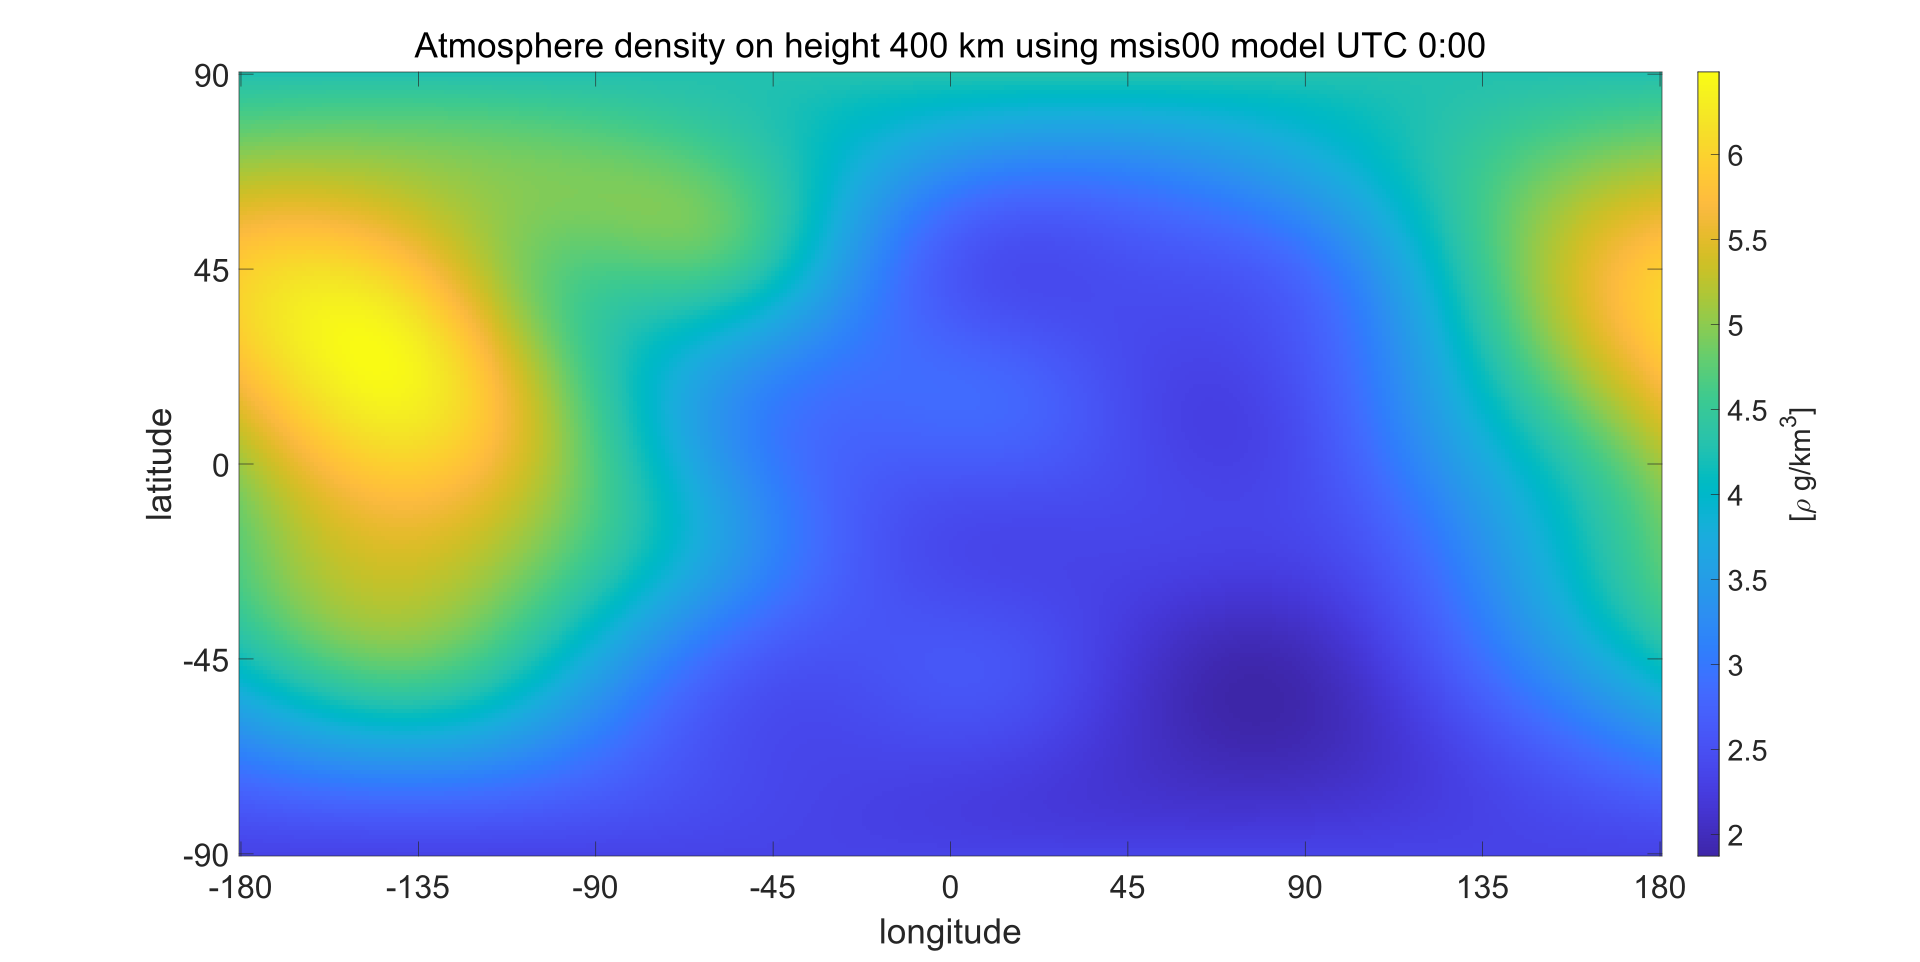
\includegraphics[width=0.9\textwidth]{images/msis_day.png}}
	\subfigure[]{
		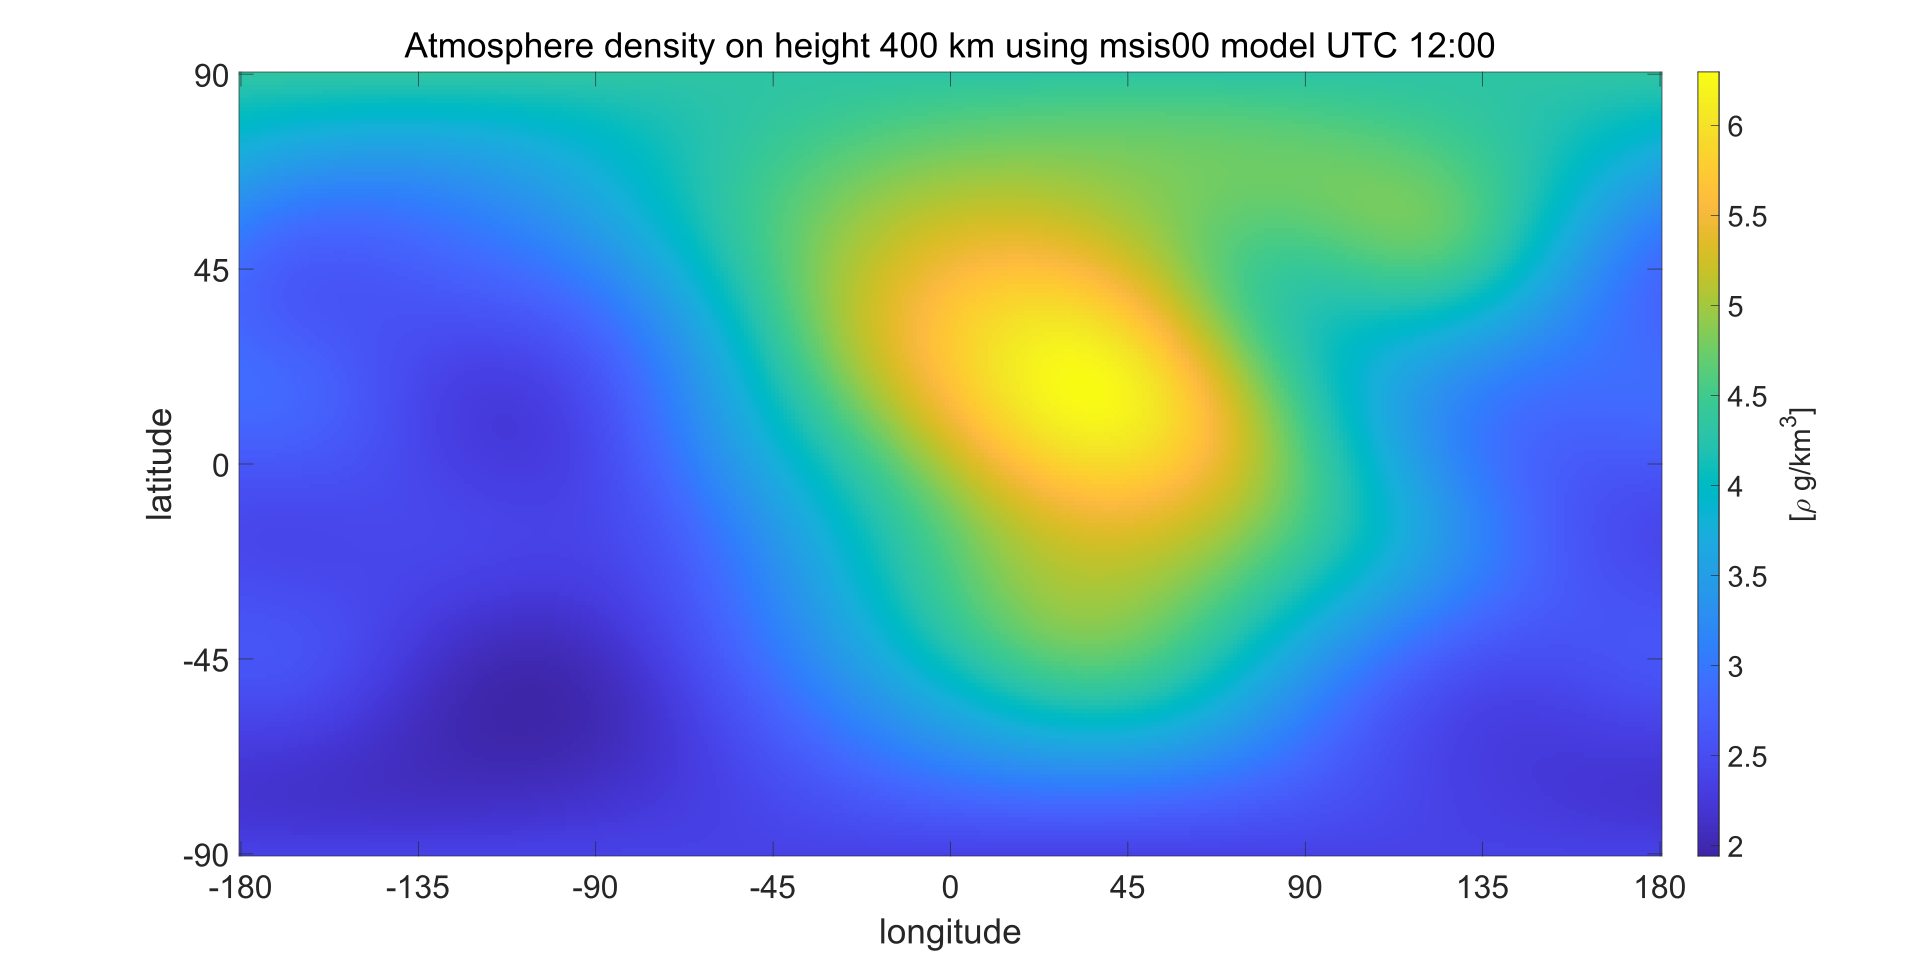
\includegraphics[width=0.9\textwidth]{images/msis_night.png}}
	\caption{Atmosphärische Dichte \SI{400}{\kilo \meter} über die Erde um 0:00 und 12:00 UTC}
	\label{fig:msise00_400km}
\end{figure}
\\
In \autoref{fig:compare_model} wird die Differenzen zwischen beiden Modellen dargestellt. Die Dichte von Harris-Priester Modell sind größer als die von MSIS-E-00 Modell sowohl über Nordpol als auch über Äquator. Außerdem sinkt die Differenz zwischen beiden Modellen mit steigende Höhe.
\\\\
In Praxis dauert die Bahnintegration ziemlich lang mit MSIS-E-00 Modell. Damit man die Zeit sparen und mehr Ergebnisse kriegen kann, verwendeten wir Harris-Priester Modell, obwohl MSIS-E-00 präziser ist.
\begin{figure}[ht]\centering 
	\subfigure[]{
		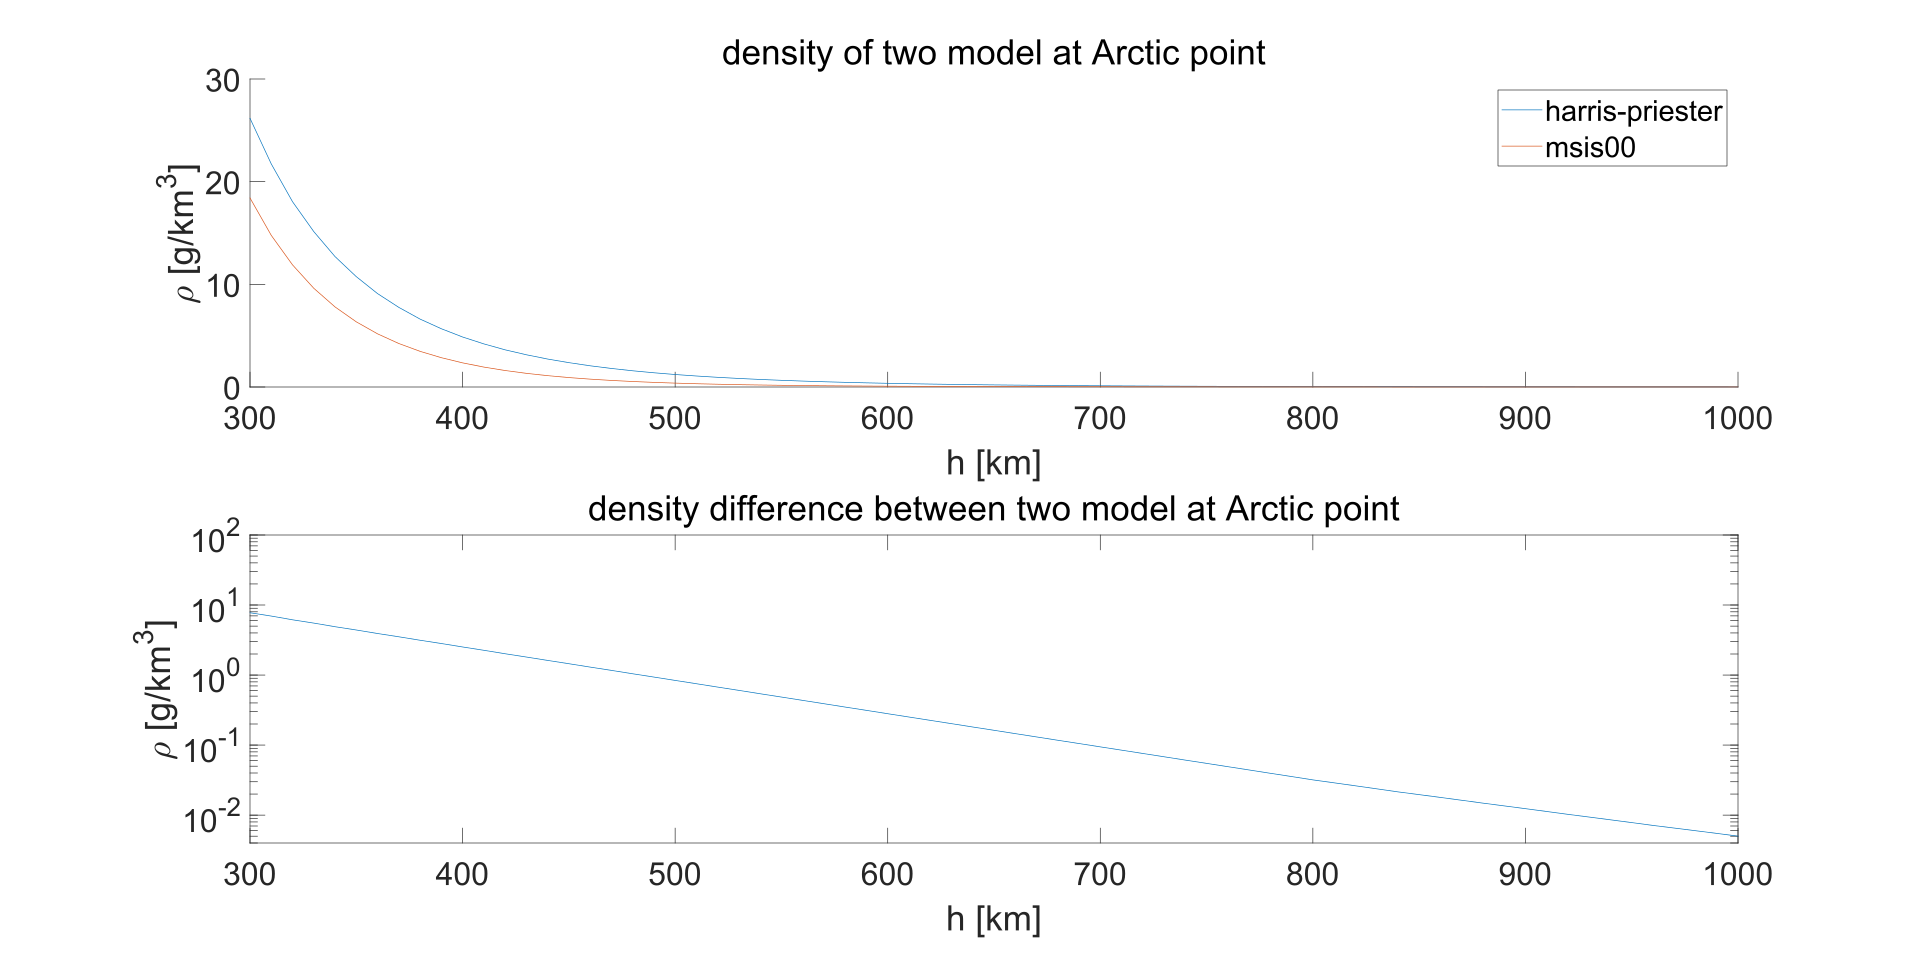
\includegraphics[width=0.9\textwidth]{images/compare_arctic.png}}
	\subfigure[]{
		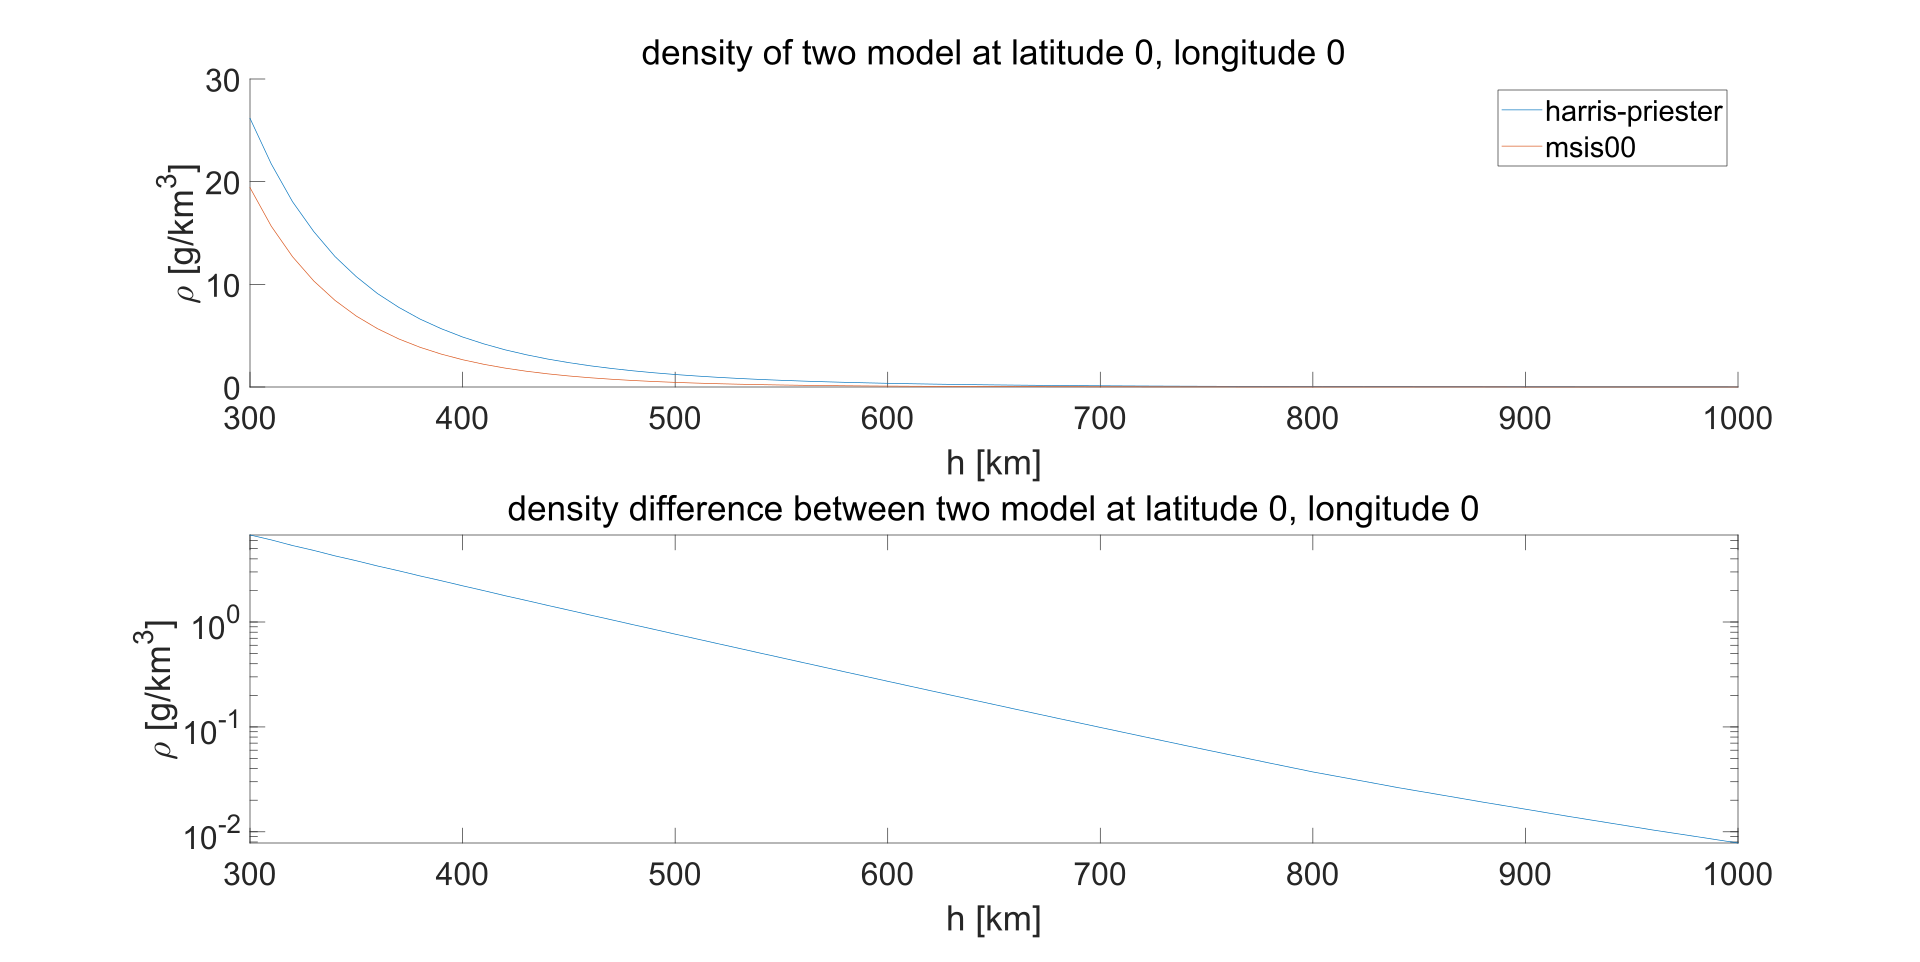
\includegraphics[width=0.9\textwidth]{images/compare_equa.png}}
	\caption{Differenzen zwischen 2 Atmosphärischen Modellen über Äquator und Nordpol}
	\label{fig:compare_model}
\end{figure}
\subsection{Andere Vereinfachung}
Satellitenbahnen werden mit nummerische Integration mit folgende Differenziale Gleichung gelöst:
\begin{equation}
	\frac{d}{dt} \begin{pmatrix}
		\bm{r} \\
		\bm{\dot{r}}
	\end{pmatrix} = \begin{pmatrix}
	\bm{\dot{r}} \\
	- \frac{GM}{r^3} \cdot \bm{r}
\end{pmatrix} + \begin{pmatrix}
\bm{0} \\
\frac{\bm{f}}{m}
\end{pmatrix}
\end{equation}
Die Störkraft $\bm{f}$ enthaltet Luftwiderstand, Solardruck usw. Da wir uns in LEO Objekten interessieren, sorgen wir nur für die atmosphärische Widerstand. Die Erde geltet als eine Kugel, daher ignoriert man die Einfluss von Erdeabplattung. Während ein Objekt um die Erde fliegt, variiert sich die Querabschnittsfläche entlang Flugrichtung wegen Kraftmoment, wir nehmen diesen Wert als einen Konstant. Die Atmosphäresgeschwindigkeit setzen wir $0$, das bedeutet, es gibt keine relative Geschwindigkeit zwischen Atmosphäre in LEO Bereich und Erde. Da wir Harris-Priester Modell verwenden, hängt die Atmosphäresdichte nur von der ellipsoidische Höhe ab, und weil wir die Erde als eine Kugel betrachtet, berechnen wir die Höhe mit folgendem Formel statt die Transformation von Kepler Elements nach Länge, Breite und Höhe zu berechnen.
\begin{equation}
	h = \lVert \bm{r} \rVert - R
\end{equation}
$R$ ist die Erdradius. Unterschiedliche Objekten haben verschiedene $C_d$ Werte, in der Simulation nehmen wir $2.5$. Danach führen wir die numerische Integration mit Hilfe von ode113 Funktion in Matlab.
\clearpage
\subsection{Integrationsergebnisse}
Unterschiedliche Anfangssituationen werden untersucht.
\subsubsection{Kreisbahn}


\clearpage
\bibliography{bib/bib.bib}
\end{document}



